\documentclass[11pt,a4paper]{article}
\author{Michael James, 390198}

\usepackage[left=20mm,right=20mm,top=20mm,bottom=20mm]{geometry}
\usepackage[pdftex]{graphicx}
\usepackage[hyphens]{url}

\begin{document}

\title{Project 1: Approximate String Search for Geolocation of Tweets}
\maketitle

\section{Introduction}
Efficient and effective approximate string matching has had a profoundly positive impact on modern society. Sophisticated approximate string matching techniques have greatly improved the ability for information identification and retrieval and have revolutionised how various industries cooperate.\\\\
The objective of Project 1 was to identify location names (ASCII strings) present within the body of a Tweet (an ASCII string between 1 and 140 characters in length). Variants of Global Edit Distance (Needleman-Wunsch) and Local Edit Distance (Smith-Waterman) matching algorithms were explored in Project 1. 

\section{Preprocessing Input Data}  

Several heuristics were employed in the preprocessing of the tweets and locations input files to improve the performance of the string approximation algorithms explored in Project 1.\\\\
The reduction in the size of the input tweet and locations files, due to the preprocessing steps outlined below, are summarised in Table \ref{table:input-table}.

\subsection{Lowercase Input and Removal of Non-Alphabetic Characters (Excluding Space)}
\label{subsec:alpha}

To reduce the sample space and as specified as a requirement of the project specification, all non-alphabetic characters, excluding space, were removed from the body of the tweets. Additionally, all alphabetic characters within a tweet were made lower case. After this stage of tweet preprocessing it would have been impossible for a location name with non-alphabetic characters and/or uppercase letters to match a substring within any tweet bodies. Therefore, non-alphabetic characters were removed from the locations list and the alphabetic characters within the locations list were made lower case to ensure the location names remained consistent with the modified tweet bodies.

\subsection{Word Stemming}

Stemming is the process of reducing inflicted words to their stem (base form).A Porter Stemmer algorithm was used in the preprocessing of the location and tweet files. \\\\
The Porter Stemmer algorithm was found to further distort a subset of misspelled words within the tweet bodies, however the Porter Stemmer was also capable of (partially) correcting miss-spelled location words. Further, the Porter Stemmer reduced the sample space of the problem by introducing consistency in tweet words referring to the same location.\\\\
A sample of differences between tweet and location strings with and without the Porter Stemmer preprocessing step can be seen in Tables \ref{table:stem-tweet} and \ref{table:stem-location}.
   
\begin{table} [h]
\caption{Stemming Tweets}
\begin{center}
	\begin{tabular}{| c | p{5.5cm} | p{5.5cm} |}
	\hline
	  & \multicolumn{2}{|c|}{\textbf{Tweet Text}}\\
	\hline
	\textbf{No Porter Stemming} &  hanh khangs wedding friends going fabulous night & foursquare made breakfast meeting morning bit interesting usual\\
	\hline
	\textbf{Porter Stemming}  & hanh khang wed friend fabul night & whi foursquar made breakfast meet thi morn bit interest usual\\
	\hline
	\end{tabular}
\end{center}
\label{table:stem-tweet}
\end{table}

\begin{table} [h]
\caption{Stemming Locations}
\begin{center}
	\begin{tabular}{| c | c | c | c | }
	\hline
	 &  \multicolumn{3}{|c|}{\textbf{Location Text}}\\
	\hline
	\textbf{No Porter Stemming} & aaa advanced air ambulance
& miami lakes & new york\\
	\hline
	\textbf{Porter Stemming} &  aaa advanc air ambul
& miami lake & new york\\
	\hline
	\end{tabular}
\end{center}
\label{table:stem-location}
\end{table}

\subsection{Removal of Stop Words And Excess White Space}
A large amount of tweets and locations contained words which were less than 3 characters in length and words which were extremely common in the English language (especially after preprocessing stage \ref{subsec:alpha}). Common words and words of one to two characters of length carried little entropy when determining whether the Twitter user was Tweeting about a location or using the words in another context (Table ).\\\\
Words of one-two characters and common words were removed from both the tweets and the locations list to further reduce processing time and avoid false positives. The list of stop words contained within the NLPK library for python was used to remove stop words from he locations and tweet texts.\\\\
It is worth noting that stop words can cause problems when searching for phrases (location names) that include them. However, after examination of the location and tweet files it was determined that the benefits of removing stop words outweighed the removal of an insignificant amount of location names. 

\begin{figure}[h]
	\centering
	\caption{Location Name Matches Before Stop Word And Small Word Removal}
	%\includegraphics[scale=0.3]{vpn/vpn2.png}
\end{figure}

\subsection{Removal of Similar Locations}
After thorough inspection of the locations file, significant overlap between the start of many location strings could be seen. To further reduce the sample size of locations, locations which had their first two words or more in common were combined into one location containing the common substring.

\begin{figure}[h]
	\centering
	\caption{Significant Repeat in Location Names}
	%\includegraphics[scale=0.3]{vpn/vpn2.png}
\end{figure}

\subsection{Removal of Duplicate Locations}       
After performing the preceding preprocessing steps, the locations list contained various duplicate entries. The duplicate locations were removed to avoid using algorithm processing time on the duplicates.

\begin{table} [th]
\caption{Input Data Size Reduction}
\begin{center}
	\begin{tabular}{| c | c | c |}
	\hline
	 &  \textbf{Word Count} & \textbf{Number of Locations}\\
	\hline
	\textbf{Raw Locations Input File} & 6,147,265 & 2,153,222\\
	\hline
	\textbf{Final Locations Input File} & 2,107,408 & 834,250\\
	\hline
	 &  & \\
	\hline
	\textbf{Raw Tweets Input File} & 66,491,876 & N/A\\
	\hline
	\textbf{Final Tweets Input File} & 37,143,754 & N/A\\
	\hline
	\end{tabular}
\end{center}
\label{table:input-table}
\end{table}

\section{String Approximation Algorithms}

\subsection{Needleman-Wunsch Global Edit Distance}

\textbf{Needleman-Wunsch}, N-W, is a popular dynamic programming algorithm for calculating the edit distance between two strings. An edit distance is a metric for quantifying how dissimilar two strings are to one another. Edit distance functions associate a cost associated with insertion, deletion, replacement and matching of characters for conversion of one string into another string. The N-W algorithm implemented in project 1 used a \textbf{Levenshtein Distance} cost function to assign a cost of 1 for insertions, deletions and replacements and a cost of 0 for matches.

\subsubsection{N-W Baseline Implementation}

The baseline (naive) method of N-W implementation involved comparing the whole body of tweet text against a location.\\\\
The run time of the N-W Baseline algorithm was extremely fast, with an average processing time of 2.884 seconds per tweet (see Figure \ref{figure:times-graph} for comparison of algorithm run times).\\\\ 
This naive solution yielded poor matching results (Table X). The poor results can be attributed to the significant difference in the location (query) length compared to the length of a tweet. The significant disparity between the length of the query strings and the tweet bodies resulted in a large number of deletions to obtain a conversion between strings, resulting in an unacceptably high Levenshtein Distance.\\\\
The scalability of N-W Baseline...

% insert tables and figures supporting argument and maths


\subsubsection{N-W Word Tokens Implementation}

To avoid the lack of matches associated with comparing location and tweet bodies of vastly different lengths the location queries and tweet bodies were tokenised into words. A location of word length N was compared with sub-strings of length N that made up a tweet body.\\\\
This brutforce style algorithm had better matching capabilities as seen in the tweet exerts of Table xxxx. However, the running time of N-W Word Tokens was significantly larger, with an average run time of 17.49 seconds per tweet (Table \ref{figure:times-graph}).\\\\
The scalability of N-W Word Tokens...

% Add tables and table references and mathamatical analysis

\subsection{Local Edit Distance}

\subsection{Needlemen-Wunsch and Smith-Waterman Combined}

Global Edit Distance 

\section{Results}

\begin{figure}[ht]
	\centering
	\caption{Comparison of Algorithm Run Times (per Tweet)}
	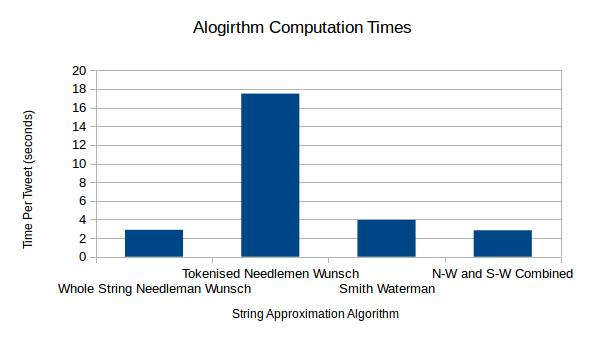
\includegraphics[scale=0.8]{times1.jpg}
	\label{figure:times-graph}
\end{figure}

\begin{table} [ht]
\caption{Sample Tweet And Matches}
\begin{center}
	\begin{tabular}{| p{5.5cm} | p{10cm} |}
	\hline
	\multicolumn{2}{|p{15.5cm}|}{\textbf{Tweet Text:} hire famili practic physician tricar outpati clinic clairemont mesa stg int httpbitlygbqg job shjob} \\
	\hline
	\textbf{Algorithm} & \textbf{Match-Score Pairs}\\
	\hline
	Baseline Needlemen-Wunsch & \\
	\hline
	Brutforce Needlemen-Wunsch & ('clairemont', 100), ('clairmont', 95), ('claremont', 95), ('clinic', 100), ('hire', 100), ('job', 100), ('mesa', 100)\\
	\hline
	Waterman-Smith & ('acti', 1.0), ('ami', 1.0), ('clair', 1.0), ('clairemont', 1.0), ('cli', 1.0), ('clinic', 1.0), ('emon', 1.0), ('hire', 1.0), ('job', 1.0), ('lair', 1.0), ('mesa', 1.0), ('mon', 1.0), ('mont', 1.0), ('pat', 1.0), ('remo', 1.0)\\
	\hline
	N-W and S-W Combined & ('acti', 1.0), ('ami', 1.0), ('clair', 1.0), ('clairemont', 1.0), ('cli', 1.0), ('clinic', 1.0), ('emon', 1.0), ('hire', 1.0), ('job', 1.0), ('lair', 1.0), ('mesa', 1.0), ('mon', 1.0), ('mont', 1.0), ('pat', 1.0), ('remo', 1.0)\\
	\hline
	Token Set Alignment & ('clairemont', 100), ('clinic', 100), ('famili clinic', 100), ('famili physician clinic', 100), ('hire', 100), ('job', 100), ('mesa', 100), ('physician clinic', 100)\\
	\hline
	\end{tabular}
\end{center}
\label{table:alg-table}
\end{table}

\section{Conclusion}


\begin{thebibliography}{9}

\bibitem{lamport94}
  Leslie Lamport,
  \emph{\LaTeX: a document preparation system}.
  Addison Wesley, Massachusetts,
  2nd edition,
  1994.

\end{thebibliography}

\end{document}